\begin{pastexam}[label={px:gw3-101-ds-05}]{關務三等資訊處理 101 年 第五題}
（申論）

㈠資料壓縮可以減少資料儲存空間或網路資料傳輸量，文字資料常使用霍夫曼編碼（Huffman coding）作壓縮。在文件中
現有六個文字訊息 A, B, C, D, E, F，其出現的次數各為 16, 12, 9, 6, 7, 2。請建立霍夫曼樹，並列出 A, B, C, D, E, F
的霍夫曼碼。㈡將收到的 1001010101001011110010111100 字串解碼，列出文字訊息。（20 分）

［註 1：建立霍夫曼樹時，比重較小的子樹成左邊子樹，比重較大的子樹成右邊子樹。\\
\phantom{［}註 2：當編碼時，左邊（left edge）是 0，右邊（right edge）是 1。］
\end{pastexam}

\begin{pastsoln}
答案：㈠ A = 11、B = 01、C = 00、D = 1011、E = 100、F = 1010；㈡ EFFBBAEDAC。

\textbf{㈠ 建樹}（資結書第~19.3~節、虛擬碼~19.3）。 每次取出比重最小的兩棵樹合併，較小的放左邊（註 1）：
\begin{center}
\begin{tabular}{clll}
\toprule
步驟 & 取出的兩棵（左、右） & 合併後 & 剩下的比重 \\
\midrule
開始 & & & F2、D6、E7、C9、B12、A16 \\
1 & F(2)、D(6) & 8 & E7、8、C9、B12、A16 \\
2 & E(7)、\{F,D\}(8) & 15 & C9、B12、15、A16 \\
3 & C(9)、B(12) & 21 & 15、A16、21 \\
4 & \{E,F,D\}(15)、A(16) & 31 & 21、31 \\
5 & \{C,B\}(21)、\{E,F,D,A\}(31) & 52 & 52 \\
\bottomrule
\end{tabular}
\end{center}
每一步取出的兩個比重都不相等，沒有平手要處理，樹是唯一的。
\begin{center}
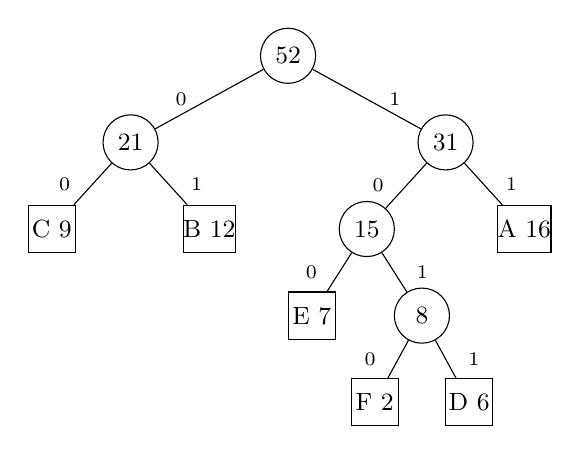
\begin{tikzpicture}[every node/.style={circle,draw,minimum size=7mm,inner sep=0pt,font=\small},
  lf/.style={rectangle,minimum size=6mm},
  e/.style={draw=none,rectangle,font=\scriptsize,inner sep=1pt},
  level distance=11mm, level 1/.style={sibling distance=40mm}, level 2/.style={sibling distance=20mm},
  level 3/.style={sibling distance=14mm}, level 4/.style={sibling distance=12mm}]
\node {52}
  child {node {21}
    child {node[lf] {C 9} edge from parent node[e,left] {0}}
    child {node[lf] {B 12} edge from parent node[e,right] {1}}
    edge from parent node[e,left] {0}}
  child {node {31}
    child {node {15}
      child {node[lf] {E 7} edge from parent node[e,left] {0}}
      child {node {8}
        child {node[lf] {F 2} edge from parent node[e,left] {0}}
        child {node[lf] {D 6} edge from parent node[e,right] {1}}
        edge from parent node[e,right] {1}}
      edge from parent node[e,left] {0}}
    child {node[lf] {A 16} edge from parent node[e,right] {1}}
    edge from parent node[e,right] {1}};
\end{tikzpicture}
\end{center}
從根走到每個葉子，左 $0$ 右 $1$（註 2），得到霍夫曼碼：
\begin{center}
\begin{tabular}{lcccccc}
\toprule
字元 & A & B & C & D & E & F \\
次數 & 16 & 12 & 9 & 6 & 7 & 2 \\
霍夫曼碼 & 11 & 01 & 00 & 1011 & 100 & 1010 \\
長度 & 2 & 2 & 2 & 4 & 3 & 4 \\
\bottomrule
\end{tabular}
\end{center}
總長度 $16 \cdot 2 + 12 \cdot 2 + 9 \cdot 2 + 6 \cdot 4 + 7 \cdot 3 + 2 \cdot 4 = 127$ 位元，平均每個字元
$127/52 \approx 2.44$ 位元，比固定長度編碼（$6$ 個字元要 $3$ 位元）的 $156$ 位元少。

\textbf{㈡ 解碼。} 霍夫曼碼是前綴碼（沒有一個碼是另一個碼的開頭），從頭讀位元、在樹上由根往下走，走到葉子就輸出
那個字元、回到根：
\begin{center}
\begin{tabular}{cccccccccc}
\toprule
100 & 1010 & 1010 & 01 & 01 & 11 & 100 & 1011 & 11 & 00 \\
E & F & F & B & B & A & E & D & A & C \\
\bottomrule
\end{tabular}
\end{center}
$3 + 4 + 4 + 2 + 2 + 2 + 3 + 4 + 2 + 2 = 28$ 位元，正好用完。 訊息是 EFFBBAEDAC。
\end{pastsoln}
